\documentclass[12pt]{article} % use larger type; default would be 10pt
\usepackage[utf8]{inputenc} % set input encoding (not needed with XeLaTeX)

%%% PAGE DIMENSIONS
\usepackage{geometry} % to change the page dimensions
\geometry{a4paper} % or letterpaper (US) or a5paper or....
\geometry{margin=2cm} % or letterpaper (US) or a5paper or....

\usepackage{graphicx} % support the \includegraphics command and options
\usepackage[parfill]{parskip} % Activate to begin paragraphs with an empty line rather than an indent
\usepackage{times} % for Times Roman default font

%%% PACKAGES
\usepackage{booktabs} % for much better looking tables
\usepackage{array} % for better arrays (eg matrices) in maths
\usepackage{paralist} % very flexible & customisable lists (eg. enumerate/itemize, etc.)
\usepackage{verbatim} % adds environment for commenting out blocks of text & for better verbatim
\usepackage{subfig} % make it possible to include more than one captioned figure/table in a single float
\usepackage{pdfpages} % import pdf files
\usepackage{float} % fix position of figures

%%% HEADERS & FOOTERS
\usepackage{fancyhdr} % This should be set AFTER setting up the page geometry
\pagestyle{fancy} % options: empty , plain , fancy
\renewcommand{\headrulewidth}{0pt} % customise the layout...
\lhead{}\chead{}\rhead{}
\lfoot{}\cfoot{\thepage}\rfoot{}

\makeatletter
\renewcommand{\maketitle}{%
  {\bfseries{\scshape{\Large{\@title\par}}}}
}
\makeatother

\hyphenation{Kiwi-bank} % otherwise it may get hyphenated as Ki-wibank

%%% END Article customizations

%%% The "real" document content comes below...

\title{Lake Man Biv Receipts}

\begin{document}
  \maketitle

\begin{figure}[H]
%\centering
\begin{center}
   \includegraphics[width=13cm, angle=270]{BCTClaimLMBPly}
   % \captionof{figure}{Ply: Greymouth ITM (first item only)}
\end{center}
\end{figure}

\begin{figure}[H]
%\centering
\begin{center}
   \includegraphics[width=16cm, angle=270]{BCTClaimLMBHardware}
   % \captionof{figure}{Hardware: Ferrymead Mutre10 Mega}
\end{center}
\end{figure}

\begin{figure}[H]
%\centering
\begin{center}
   \includegraphics[width=16cm]{BCTClaimLMBTimber}
   % \captionof{figure}{Timber: Dyers Road ITM}
\end{center}
\end{figure}

%\includepdf[pages=-]{BCTClaimLMBWindowQuote.pdf}
\includepdf[pages=-]{BCTClaimLMBWindow.pdf}
\begin{figure}[H]
%\centering
\begin{center}
   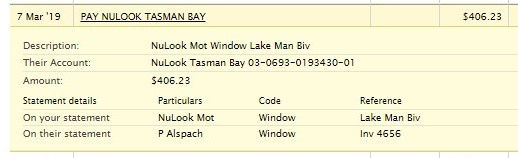
\includegraphics[width=16cm]{BCTClaimLMBWindowReceipt}
   % \captionof{figure}{Timber: Dyers Road ITM}
\end{center}
\end{figure}

\includepdf[pages=-]{BCTClaimLMBBenchtop.pdf}
\begin{figure}[H]
%\centering
\begin{center}
   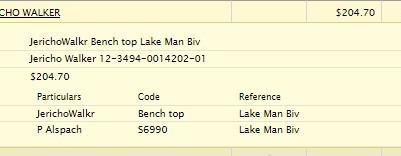
\includegraphics[width=16cm]{BCTClaimLMBBenchtopReceipt}
   % \captionof{figure}{Timber: Dyers Road ITM}
\end{center}
\end{figure}

\includepdf[pages=-]{BCTClaimLMBHelicopter.pdf}
\begin{figure}[H]
%\centering
\begin{center}
   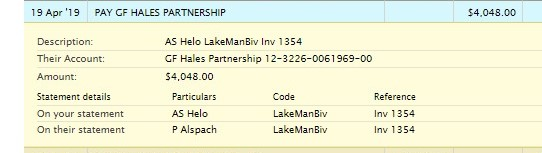
\includegraphics[width=16cm]{BCTClaimLMBHelicopterReceipt}
   % \captionof{figure}{Timber: Dyers Road ITM}
\end{center}
\end{figure}

\end{document}
